\chapter{Mesh}\label{chapter:mesh}
In this chapter the part of the code regarding the management of a grid will be explained . The code can take as input all the information about the grid stored in a \verb|GMSH| file format and distributes all the grid information among N processes in an optimal way using the \verb|ParMETIS| and \verb|METIS| libraries. Both this part of the code and the chapter regarding it have been developed by a collaboration among Marco Agnese, Francesco Boffa and Marco Chiaramello. We decided to develop this parts together because each of us solves a problem on unstructured and conformal grids. Definitions of these grids will be explained in Sec.(\ref{subsection:gmsh}). In Fig.(\ref{fig:mesh_diagram}) it is possible to see the general structure of the code and the inheritances of the classes involved.

\begin{figure}
\centering
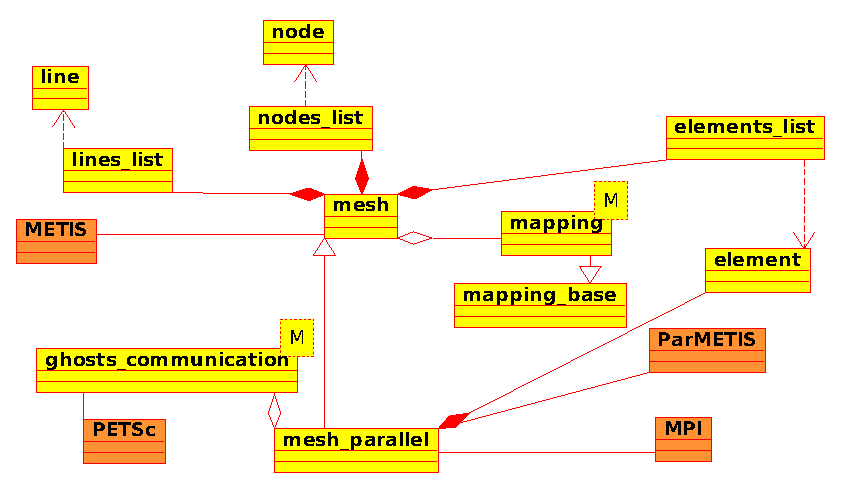
\includegraphics[scale=1]{images/mesh_diagram.eps}
\caption{Mesh management: classes structure.}
\label{fig:mesh_diagram}
\end{figure}

\section{Sequential mesh management}\label{section:mono_cpu}
The mesh management part of the code is structured in two main different classes. The class \verb|mesh| is implemented in a sequential way: its methods can be invocate in the same way when the code is run in a sequential or parallel way. Depending on which way it is run, its members will contain information of the global mesh or the local one.

The second class is \verb|mesh_parallel| and it manages the parallel methods, cmp. Sec.(\ref{section:multi_CPUs}).

\subsection{Data structures}\label{subsection:data_structures}
This part of the code involves the definition of some data structures in which all the information about the grid are stored.

\subsubsection{Nodes data structures}
The class \verb|node| contains all the methods to manage the information about the nodes of the grid. The physical coordinates are stored in a vector of \verb|double|, while the global index is stored an integer variable. A vector of classes \verb|node| is created in the class \verb|nodes_list|. The class \verb|nodes_list| contains also the methods to set the coordinates and the index of each node in the nodes list and to add an element to the vector of \verb|node|.

\subsubsection{Elements data structures}
In the class \verb|element| we have implemented all the methods necessary to completely define each element of the mesh. In particular, we have defined seven members of this class: four vectors of integers containing respectively the index of the vertex, the neighboring elements, the position of the corner elements and the relative position of the reference element on each neighboring element, and other two variables storing the global index of the element and the surface tag. The latter allows to define many different surfaces on the same domain, distinguishing the different portion. In the last variable (type: \verb|boolean|) is stored a flag which reveals if an element is a ghost or not, when the code is run in parallel. The vector of neighboring is set of variable dimension, due to the fact on a unstructured grid the number of elements neighboring a reference element is not fixed; both the elements situated on the sides and on the corner of the reference element are stored in this vector, cmp. Fig.(\ref{fig:element_neigh}) and Fig.(\ref{fig:element_corner}). The vector of position of the corner elements allows to determine, when the vector of neighboring has been created, on which corner each neighbor sharing one vertex with the reference element is located. The vector storing the relative position of the reference element on each neighboring element (called \verb|neighbor_cor_pos|) allows to reconstruct uniquely the position of each element respect to the others, regardless the orientation of each element. In the class \verb|element_list| a vector of \verb|element| is created, together with all the methods necessary to set the \verb|element| members. In the \verb|element_list| member variable called \verb|number_ghosts| is stored the number of ghosts allocated on each process, cmp. Sec.(\ref{section:multi_CPUs}).

\begin{figure}
\centering
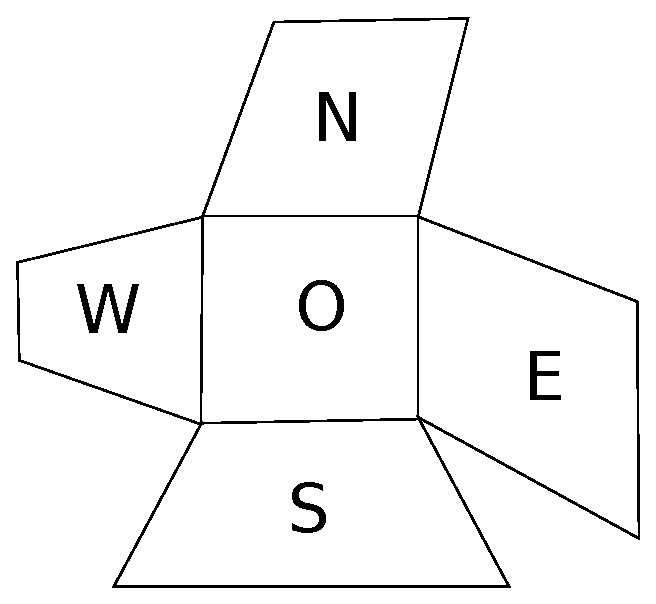
\includegraphics[scale=.45]{images/mono_cpu_data_structures_element_neigh}
\caption{Elements S,W,N,E are neighbors of element 0 located on its sides.}
\label{fig:element_neigh}
\end{figure}

\begin{figure}
\centering
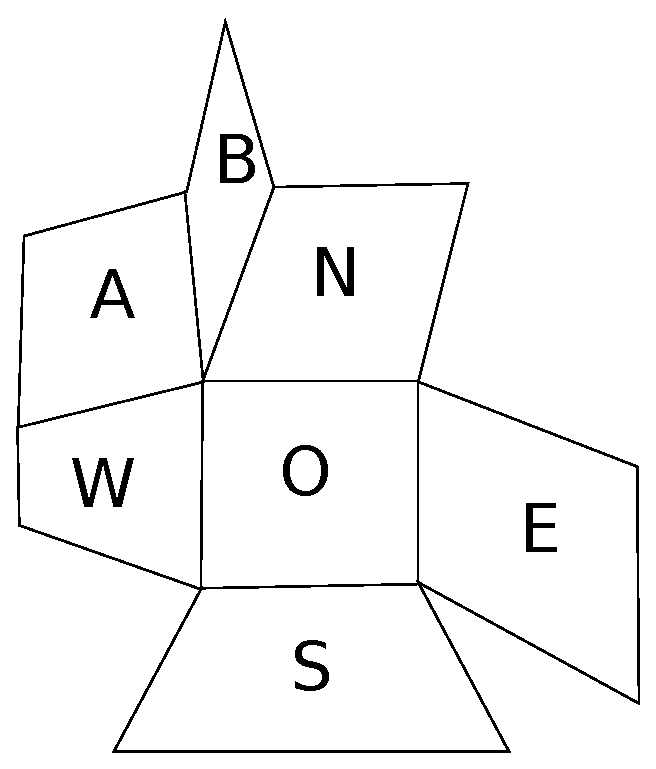
\includegraphics[scale=.45]{images/mono_cpu_data_structures_element_corner}
\caption{Elements A,B are neighbors of element 0 located on its corners.}
\label{fig:element_corner}
\end{figure}

\subsubsection{Lines data structures}
The class \verb|line| contains the methods to characterize the lines belonging to the border of the domain. In a vector of integers we store the vertexes of each line. In other four members of type \verb|int| we store the global index of the line, a tag, the index of the element to which the line belongs and the index of the side of the element in which the line is located, respectively. The tag indicates the type of boundary condition is imposed on that line. Then in the class \verb|lines_list| we create a vector of \verb|line|, together with all the methods necessary to set all the members of \verb|line|.

\subsection{Main methods involved}\label{subsection:mono_cpu_methods}
All the most important algorithms involved in the definition of the topology of the mesh are included in the class \verb|mesh|. In particular, the methods implemented in this class allows the user to read the grid information from a file (in a \verb|.msh| format ), to evaluate all the neighbors situated on each side of the reference element, to determine the elements situated on the corners, to define if an element is a border one. All these methods are reported in detail below.

\subsubsection{read\_file}
It takes as input the name of the file in which the grid information are stored. Following the \verb|GMSH| format (cmp. \ref{subsection:gmsh}), it stores the data in the classes (\verb|nodeslist|, \verb|elementslist| and \verb|lineslist|) converting from a string format to a numerical one.

\subsubsection{eval\_topology}
It reconstructs the topology of each element. This means that determines all the elements that share one or two vertexes with a reference element. This evaluation has been implemented using the command \verb|METIS_MeshToDual| of the \verb|Metis| library. All the neighboring elements are stored without making any difference if they are located on a side of the reference element or if they share a single vertex.
\medskip

For example, the vector of neighbors of the element 0 reported in Fig.(\ref{fig:mono_cpu__main_methods_involved__eval_topology}) will be:
\medskip

neighbors=[1,7,9,5,2];

\begin{figure}
\centering
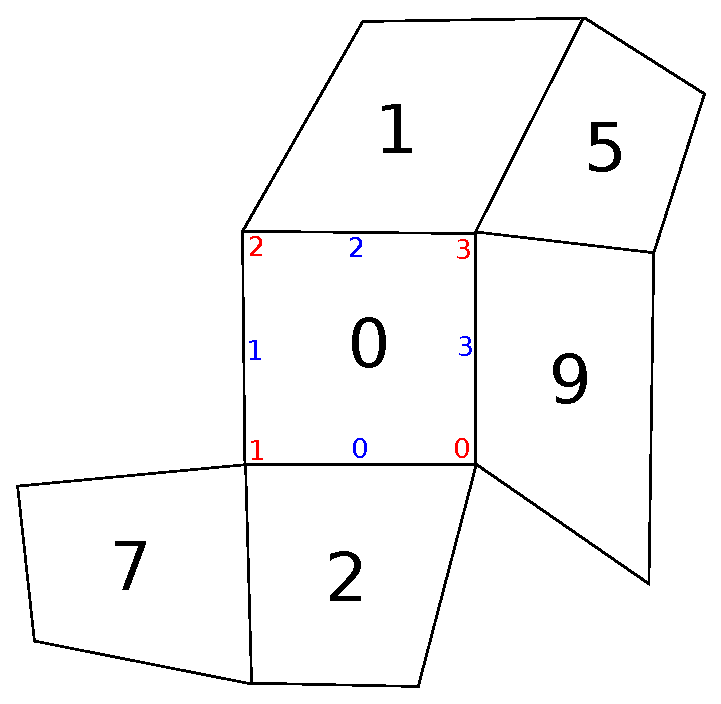
\includegraphics[scale=.45]{images/mono_cpu_main_methods_involved_eval_topology}
\caption{Example of configuration; in red local numbering of nodes, in blue local numbering of lines.}
\label{fig:mono_cpu__main_methods_involved__eval_topology}
\end{figure}

\subsubsection{reorder\_neighbors}
The neighboring elements are stored by \verb|Metis| in a not ordered way. This function reorders the neighbors in order to have the side neighboring positioned in the first four position of the neighbors vector reordered. If the reference element has less than 4 neighbors located on the edge, in the vector of the neighbors will be reported the number of the correspondent line multiplied (-1) and reduced of 1. A support vector is used as pointer to determine in which position of the vector the neighbors of the i-th corner are located.
\medskip

For example, referring to Fig.(\ref{fig:mono_cpu__main_methods_involved__eval_topology}), the reordered vector of neighboring and the vector of pointers will be:
\medskip

neighbors=[2,9,1,-4,7,5]; ptr=[4,4,5,5];

\subsubsection{set\_neighbors\_cor\_pos}
\verb|GMSH| creates a mesh orienting the elements in a pseudo random way. Considering a reference element and one of its neighbors, this function sets on which edge the reference element is located respect to the neighbor considered. In that way is possible to match uniquely the sides of the elements. This information is stored in the vector \verb|neighbor_cor_pos|, member of the class \verb|element|. It is possible to obtain this information using the method \verb|neighbor_orientation|.

\subsubsection{write\_file}
It writes all the information elaborated on each element in a \verb|.msh| format (cmp. Sec.(\ref{subsection:gmsh})). The name of the file is specified as input to the method.

\subsection{Boundary conditions}
We create a vector of vector of function pointers, called \verb|border_function_ptr|, that allows to set different boundary functions on the same region (for example, a different boundary function for each degree of freedom of the problem) or in different regions of the domain. The method \verb|set_border_function| allows the user to set these boundary functions: it takes in input the function itself, the index of the first and the last line involved, a flag referring to the type of boundary condition (\verb|DIRICHLET|, \verb|NEUMANN|, \verb|WALL|, \verb|NOCONDITION|) and the number of degree of freedom we want to set (default 1). The method \verb|get_bc_type| returns the type of the boundary condition imposed on a line while the method \verb|eval_bc| determines the value of the boundary function in a given point.

Periodicity boundary conditions deserve a particular attention. The user has to guarantee a correspondence 1 to 1 between elements periodic to each other and he must not override the line with the lower index. This condition is set using the function \verb|set_periodicity_mesh| where the lines indexes of first border are imposed in ascending order while the corresponding border is specified giving the index number of the first corresponding line and the las corresponding line. This method simply change the neighbors of the elements involved in the periodicity. Moreover it constructs the following mapping between the lines:

\begin{itemize}
\item 0, no periodic condition;
\item $i<0$, periodic with the line $-i-1$ in reverse order of the nodes;
\item $i>0$, periodic with the line $i-1$ in direct order of the nodes.
\end{itemize}

\subsection{Logical to physical transformation}\label{subsec:mapping}
It is necessary to define a transformation between a logical domain (on which the problem is solved) and the physical domain. In the following, the map from from a logical quadrangular of coordinates $[-1,1]\times[-1,1]$ to a physical one is reported:

\begin{equation}\label{eq:transf_1}
\textbf{F}_m:[-1,1]^2 \rightarrow \Omega_m \subset \mathbb{R}^2
\end{equation}
where
\begin{equation}\label{eq:transf_2}
\textbf{x}=\textbf{F}_m(\hat{\textbf{x}})= \frac{1}{4} \sum_{i=1}^{4} (1+\sigma_{\hat{x}}\hat{x})(1+\sigma_{\hat{y}}\hat{y}) \textbf{v}_i
\end{equation}
where $\textbf{x}$ are the coordinates of a point in the physical domain, $\hat{x}$ and $\hat{y}$ are the coordinates of the point in the logical domain, $\sigma_{\hat{x}}$ and $\sigma_{\hat{y}}$ are the coordinates of the reference quadrangular in the logical domain:

\begin{table}
\centering
\begin{tabular}{|c|c|}
\hline
$\sigma_{\hat{x}}$ & $\sigma_{\hat{y}}$\\
\hline
+1 & +1\\
\hline
+1 & -1\\
\hline
-1 & -1\\
\hline
-1 & +1\\
\hline
\end{tabular}
\caption{Transformation coefficients.}
\label{tab:coeff}
\end{table}

In Eq.(\ref{eq:transf_2}) the vector $\textbf{v}_i$ there are the coordinates of each vertex of a quadrangular in the physical domain. So, knowing the logical coordinate $\hat{\textbf{x}}=(\hat{x},\hat{y})$ of a point in the logical domain, it's possible reconstruct its position respect to the quadrangular of physical vertex $\textbf{v}_i$ in the physical domain. Based on this transformation, it is possible to build the Jacobian of the transformation, the determinant of the Jacobian and the inverse Jacobian. All the methods regarding the transformation from the logical domain to the physical one are implemented in the classes \verb|mapping_base| and \verb|mapping|.

\section{Parallel mesh management}\label{section:multi_CPUs}
The core part of the mesh management is contained in the class \verb|mesh_parallel| which implements all the methods necessary to obtain a good partitioning of the grid over the cluster. It is a derived class because it inherits from the class \verb|mesh|, cmp. Sec.(\ref{section:mono_cpu}). The logic behind this implementation is that all the mesh data, the I/O methods and all the methods to evaluate the topology of the mesh are implemented in \verb|mesh| which can be used alone, for a sequential code, or it becomes the base class in a parallel code. Therefore, in the case of a parallel code, each process will allocate a \verb|mesh_parallel| variable which will not contain the global informations of the mesh but only the local ones.
\medskip

In a parallel code, each process is identified by an unique positive number called $rank$. In the following we will use use the convention to call \textit{root process} the the process with $rank=0$.

\subsection{Overview of the class}\label{subsection:multi_CPU_overview}
After doing a mesh with the software \verb|GMSH|, cmp. Sec.(\ref{subsection:gmsh}), the user has to save the file in the \verb|.msh| format. The basic things that the class perform are: the class allocated on root process reads the file and loads the data in its data structures, then operates a simple pre-partitioning sending equal parts of the mesh to each process and finally operates a good partitioning redistributing the mesh over the processes. The user can decide to write on file, one for each process, the local part of the mesh obtained with the pre-partitioning and/or with the partitioning in \verb|.msh| format to avoid to recompute every time the partitioning. The constructor of the class accepts several variables to choose what the class have to do:

\begin{itemize}
 \item $1^{st}$ parameter: rank of the process;
 \item $2^{nd}$ parameter: size, therefore the number of processes available for the simulation;
 \item $3^{rd}$ parameter (default=0): number of refinements , how many times the partition  has to be refined;
 \item $4^{th}$ parameter (default=\verb|"mesh.msh"|): file name (type \verb|string|), it is the name of the input file for the mesh;
 \item $5^{th}$ parameter (default=\verb|READ_MONO|): flag that indicates the input mesh type: \verb|READ_MONO| if the root process reads the full mesh, \verb|READ_PARALLEL_PRE| if each process reads its local non optimized partitioned mesh and \verb|READ_PARALLEL_PAR| if each process reads its local optimized partitioned mesh;
 \item $6^{th}$ parameter (default=\verb|WRITE_OFF|): flag that indicates the output mesh type: \verb|WRITE_OFF| if there is no output, \verb|WRITE_PREPARTITIONING| if each process writes on file its local mesh after the pre-partitioning, \verb|WRITE_PARTITIONING| after the partitioning, \verb|WRITE_REFINEMENT| after the refinement and \verb|WRITE_ALL| after each phase. Each process save a file with is local mesh, the file name is the one given in the first parameter adding the $rank$ of the process and the suffix \textit{pre} or \textit{par} or \textit{ref} depending on the flag chosen.
 \item $7^{th}$ parameter (default=1); \verb|ncon| used as option in the function \verb|ParMETIS_V3_PartMeshKway|, cmp. Sec.(\ref{subsection:parmetis});
 \item $8^{th}$ parameter (default=2); \verb|ncommonnodes|, like parameter $7^{th}$;
 \item $9^{th}$ parameter (default=1.05): \verb|ubvecc|, like parameter $7^{th}$.
\end{itemize}
There are other 3 possible parameters to add, but the explanation will be given in the last part of this section.
\medskip

When the class is constructed, according to the constructor input variables, the mesh is partitioned over the processes and all the necessary information are evaluated therefore no methods have to be called after that. The constructor of the class \verb|mesh_parallel| performs the following operations:

\begin{enumerate}
 \item reads the mesh file using the method \verb|read_file|, class \verb|mesh.msh|;
 \item computes the mesh topology, therefore for each element it computes the surrounding squares, using the method \verb|eval_neighbors|, class \verb|mesh.msh|;
 \item sends a portion of the mesh from the root process to the other processes using the method \verb|pre_partitioning|, class \verb|mesh_parallel|;
 \item writes on file the pre-partitioned mesh using the method \verb|write_file|, class \verb|mesh.msh|;
 \item computes the new topology, like point 2;
 \item finds a better partition and redistributes the local meshes among the processes using the method \verb|partitioning|, class \verb|mesh_parallel|;
 \item computes the new topology, like point 2;
 \item writes on file the partitioned mesh, like point 4;
 \item performs some refinements using the method \verb|refinement|, class \verb|mesh_parallel|;
 \item writes on file the refined mesh,like point 4;
 \item reorders the neighbors in a proper way using the method \verb|reorder_neighbors|, class \verb|mesh|;
 \item set for each line the global index and the local position of the element that contains the line using the method \verb|eval_border|, class \verb|mesh|;
 \item set for each element its position respect to its neighbors using the method \verb|set_neighbors_cor_pos|, class \verb|mesh|;
 \item creates the mapping of the ghosts using the method \verb|create_ghosts_mapping|, class \verb|mesh_parallel|.
\end{enumerate}

It is important to notice that the methods \verb|reorder_neighbors|, \verb|eval_border|, \verb|set_neighbors_cor_pos| and \verb|create_ghosts_mapping| are used only at the end since those information are not used during the pre-partitioning, partitioning and refinement phases.

\subsection{Principal methods}\label{subsection:multi_CPU_methods}
To better understand how all these operations are performed, we now explain how the principal methods have been implemented. We use the \verb|MPI| library, cmp. Sec.(\ref{subsection:mpi}), or \verb|PETSc| library, cmp. Sec.(\ref{subsection:PETSc}),for all the methods which perform parallel communication.

\subsubsection{Pre-partitioning}
The pre-partitioning is performed by the method \verb|pre_partitioning|. The goal of this method is to split and distribute the initial mesh loaded on root process in a uniform way, from the point of view of number of elements, among all the processes. It is important to notice that only the elements are distributed among the processes while each process owns a copy of the whole \verb|nodes_list| and \verb|lines_list|. Obviously this approach is not optimal for what concern the memory usage because there are data duplications; moreover it implies a lot of communication among the processes. On the other hand, it is not necessary to find which nodes and lines has to be sent to each process, operation quite expensive, and it is not necessary to create a mapping. Finally, having a copy on each process, means that it is not necessary to compute and send these information each time that the partition changes but only during the pre-partitioning. Therefore the gain is bigger than the drawback in general; obviously,
if there are problem of memory availability, the first solution should be preferred.
\medskip

For what concerns the \verb|nodes_list|, we use the function \verb|MPI_Bcast| to send the data from the root process to the others. The sender packs the data into two different buffers: one of type \verb|double| containing the coordinates of all the nodes and the other of type \verb|int| containing their global index. The receivers unpack the buffers storing the information in their local \verb|nodes_list|. Before this step it is necessary to know the size of the buffers to send, therefore the number of nodes is broadcasted to each process. The broadcasting of the \verb|nodes_list| is exactly the same except that now the buffer is only one due to the fact that all the data are integer.
\medskip

The preliminary step for the splitting the \verb|elements_list| over the processes is to decide the destination of each element. We use a very simple method to do this: we divide the \verb|elements_list| into blocks of almost equal size each containing a consecutive sequence, considering the \verb|global_index|, of elements and each block is assigned to one process. The pros of this method are that it is very fast and simple to implement, the cons are that close indexes doesn't mean close elements because the \verb|GMSH| numbering is quite random and therefore the resulting pre-partition is usually very inefficient. It is necessary that each process knows which elements will receive, therefore we create a vector with the structure of the \verb|ParMETIS| \verb|elmdist| and we broadcast them to each process; with the information contained in the \verb|elmdist|, each process knows exactly the number and the global indexes of the elements that it will receive. Then the root process packs all the data of one
block in a buffer of \verb|int| and sends it to the corresponding process using the function \verb|MPI_Send|, while the receiving process receives the data using the function \verb|MPI_Receive| and unpacks the buffer. It is important to notice that the data contained in the buffer are always different and, since it is use only one buffer, it is necessary to use a blocking communication to avoid loss of data.
\medskip

It is necessary that each process stores not only its own elements but also the ghosts elements to evaluate in a proper way the mesh topology using the function \verb|eval_topology|. Ghost elements are the neighboring elements which do not belong to the process. They are necessary otherwise, the topology evaluation, instead of neighbors, would find border. After evaluating the ghosts, like for the elements, we scatter the number of ghosts to send and then the buffer of ghosts.
\medskip

Obviously, the root process has the data of the whole mesh therefore at the end all the elements which belongs to other process must be free.

\subsubsection{Partitioning}
In general the pre-partitioned mesh is an ensemble of disjointed clusters of elements and therefore it is quite inefficient to perform calculations on such domains because it implies a lot of communication and a consequent waste of time. For this reason it is necessary to repartition the mesh in a way that each process own only a connected cluster of elements to ensure a minimal number of ghosts elements.

The \verb|ParMETIS|, cmp. Sec.(\ref{subsection:parmetis}), function \verb|ParMETIS_V3_PartMeshKway| evaluates a better partitioning knowing the initial mapping of the elements. The output is a local mapping which maps each element to a certain process. Given this mapping the function \verb|partitioning_move_elements| physically moves the elements among the processes.
\medskip

Every process keeps a certain amount of elements and receives all the other from other processes; it is very inefficient to perform a direct substitution in its \verb|elements_list| since it is necessary to be sure not to overwrite elements which have not already been moved, otherwise it could happen a data loss. The direct substitution could be implemented storing a flag in each element to indicate if that element has already been moved or not: if it has not been moved yet, that element have to be stored in a temporary variable to avoid the overwriting.

This mechanism works but it is not very efficient because the number of elements to move is generally very large indeed it is almost the same order of magnitude of the elements present in the process. We adopt the solution to create a new \verb|elements_list| for each process to store the elements received. The previous \verb|elements_list| is destroyed and substitute with the new one at the end of all the communications. The inefficiency of this method is that it is necessary to perform a copy of the elements which are mapped in the same process. Instead of using \verb|MPI_Send| and \verb|MPI_Receive| for what concern the communication each process communicates how many elements will it send to the other process using the function \verb|MPI_Scatter| and after it sends a buffer of elements with the function \verb|MPI_Scatterv|. Each process receives the number of elements and the buffer calling the same functions. These functions are both blocking, therefore, starting for process with $rank=0$ until the
highest $rank$ one process scatters its elements and all the others receive; until process with $rank=n$ has finished to send and all the other processes have finished to receive, process with $rank=n+1$ can't start. The blocking communication is not the fastest because some processes have to idle to wait the others but it avoid problems of overwriting and data losses.
\medskip

After the scattering of the elements, in a similar way, each process scatters the ghosts.

\subsubsection{Refinement}
The mesh partitioning obtained with \verb|ParMETIS_V3_PartMeshKway| is not optimal but can be refined with the function \verb|ParMETIS_V3_RefineKway| that asymptotically converges to the optimal partitioning. This function does not work with a mesh but it is necessary to create the dual graph using \verb|ParMETIS_V3_Mesh2Dual| and than using the output dual graph as input of the refinement function. As seen before, the re-mapping provided by \verb|ParMETIS| is used by the method \verb|partitioning_move_elements| to physically move the elements among the processes.

Since \verb|ParMETIS_V3_RefineKway| is an iterative algorithm which can be called an arbitrary amount of time, it is necessary to recompute the mesh topology and the \verb|elmdist| each time at the end of each iteration.

\subsubsection{Ghosts' Mapping}\label{subsection:ghost_mapping}
Each process stores only a certain part of the mesh, therefore it is necessary to have a way to know which process owns a certain information. To perform this task it is required to have a mapping. There are in general two types of mapping:

\begin{itemize}
\item \textit{local to global}: it returns the global index knowing the local index;
\item \textit{global to local}: it returns the process and the local index knowing the global index;
\end{itemize}

Since each element contains its global index, the local to global mapping is already present. Instead, for what concern the local to global one, it is necessary to know it only for the ghost elements. The method \verb|create_ghosts_mapping| create this mapping which consists, for each ghost, in the rank of the process which stores the element and its local position. The evaluation of this mapping is very simple since it is based on the class \verb|ghost_communicaton|: each process set for each elements its own rank and the local position and then the class perform all the necessary communication. Each process stores its mapping in a vector and it is possible to know the rank and the position of a certain ghost using the functions \verb|get_ghosts_rank| and \verb|get_ghosts_pos|.

\subsubsection{Set Periodicity condition}\label{subsection:set_periodicity}
The periodicity condition when it is set for a parallelized mesh is slightly different from the sequential case since it is possible that the periodic elements are stored partly or completely in an other process. The function \verb|set_periodicity| first call the function \verb|set_periodicty_mesh| of the class \verb|mesh| which add all periodic elements like ghosts if they are not locally stored and change simply the neighbors information for the others. But this method add these ghosts with only the information of their global index because when it is used only on a single process there will be no need to add new ghosts since the process stores all the mesh. Therefore the function, in the parallel class, use the class \verb|ghost_communicaton| to obtain all the information needed for this new ghosts, namely the vertex global index. This operation is performed simply setting on each process and for each elements the four vertex information and storing the ghosts values after the class has performed the
communication.

\subsection{Class ghost\_communication}\label{subsection:ghost_communication}
The class mesh contains as member a pointer to the class ghost\_communication. This class has the purpose of providing methods to update the values needed in ghost elements. It relies completely on \verb|PETSc| functions which will be explain in detail in  Sec.(\ref{subsection:PETSc}).

The class is built in a way that it is easily possible to change the amount of data which has to be communicated per element by the call of a single function. This is a very desirable feature, because it can be used for different purpose and the user doesn't have to deal with \verb|PETSc| functions every time. In fact the constructor creates the local \verb|PETSc| vec which will contain the values on the processor and the ghost values after being updated. Then it is mandatory to call the function \verb|set_size| before using it the first time and every time one wants to change the number of values per element. This function calls first \verb|set_idxs| which sets the arrays of indices needed by the \verb|PETSc| function \verb|VecCreateGhost|, which is called right after, and needed to set local values and retrieve local ghost values. In this way a global ghosted vector is created.

To update ghost values it is sufficient to call the function \verb|set_global_vec| passing to it a vector of local values which contains the values for the actual elements on the processor. This functions contains the calls to \verb|PETSc| functions:

\begin{itemize}
\item \verb|VecSetValues|;
\item \verb|VecAssemblyBegin|;
\item \verb|VecAssemblyEnd|;
\item \verb|VecGhostUpdateBegin|;
\item \verb|VecGhostUpdateEnd|;
\item \verb|VecGhostGetLocalForm|;
\item \verb|VecGetValues|;
\item \verb|VecGhostRestoreLocalForm|.
\end{itemize}

After this sequence the private member \verb|ghost_values| contains the updated values and to retrieve them it is possible to call the public functions \verb|get_ghosts_values| to obtain a reference to all the vector and  \verb|get_ghosts_value| to obtain a reference to the element specified during the call.

The implementation allows the user to communicate only \verb|double| values.

It is also possible to specify two indices of the local vector,where to start and end to fill the global \verb|PETSc| Vec.

The function \verb|free| is provided to free the memory from \verb|PETSc| variables when not needed anymore.

\section{Libraries and tools}\label{section:lib}
In this section different libraries and free software used for the code are explained.

The mesh generation is performed using \verb|GMSH|, while \verb|METIS| and \verb|ParMETIS| are used to evaluate neighboring squares and compute an optimized partitioning of the elements among the processes.

\verb|MPI| is used to actually send data to processes according to the partitioning previously computed.

\verb|PETSc| provides the functions to update ghosts' values and it is used to obtain information about periodic ghost elements.

Functions of interest are shown for each library and the logic behind their algorithms is analyzed.

\subsection{GMSH}\label{subsection:gmsh}
The mesh is generated with the free software \verb|GMSH|. This software is a tool to create meshes in both bi-dimensional and tri-dimensional domains. In this section we give a little presentation of the software. For further information cmp. \cite{gmsh_man} and \cite{gmsh_art}.

Before explaining the software some useful definitions are given:

\begin{itemize}
\item \textit{Structured grid}: grid built with a tassellation of n-dimensional Euclidean space by congruent parallelotopes\cite{wolfram_struct}.
\item \textit{Unstructured grid}: tassellation of an Euclidean domain by simple shapes in irregular pattern.
\item \textit{Conformal grid}: grid where each node of each element is in correspondence of nodes of other elements. In such a grids there are no nodes on element edges.
\item \textit{Unconformal grid}: nodes on elements edges are allowed.
\end{itemize}

The software allows the drawing of a geometry as set of points and lines which connect these points. Once the geometry is drawn as a closed set of lines it is sufficient to create a plane surface inside it and then generate the mesh. It is also possible to give the initial geometry as input if one knows the \verb|GMSH| format, which will be explained later. In fact it is possible to write a textfile in the format \verb|.msh| in which only the points, or the points and the lines connecting them are written. \verb|GMSH| can read this kind of files and build up the initial geometry on which the mesh is then generated.

For the purpose of this work we used only meshes which contain quadrangular elements. In our code we use always a clockwise ordering of the vertexes of each element. To respect this convention, it is necessary to draw the geometry using a clockwise sense.

\verb|GMSH| gives the possibility to choose between three different algorithms for the creation of the first coarse mesh. In each of them a Delaunay mesh that contains all the points of the initial geometry is first constructed using a divide-and-conquer algorithm. Missing edges are recovered using edge swaps. After this initial step three different algorithms can be applied to generate the final mesh:

\begin{itemize}
\item \textit{Delaunay} algorithm in which new points are inserted sequentially at the circumcenter of the element that has the largest adimensional circumradius. The mesh is then reconnected using an anisotropic Delaunay criterion.
\item \textit{MeshAdapt} algorithm is based on local mesh modifications. This technique makes use of edge swaps, splits, and collapses: long edges are split, short edges are collapsed, and edges are swapped if a better geometrical configuration is obtained.
\item \textit{Frontal} algorithm is inspired by the work of S. Rebay, which is based on a Delaunay triangulation, but computes simultaneously point positions and connections.
\end{itemize}

The three different algorithms are ranked in Tab.(\ref{tab:rank}):

\begin{table}
\centering
\begin{tabular}{|l|c|c|c|}
\hline
 & Robustness & Performance & Element quality\\
\hline
\verb|MeshAdapt| & 1 & 3 & 1\\
\hline
\verb|Delaunay| & 2 & 1 & 2\\
\hline
\verb|Frontal| & 3 & 2 & 1\\
\hline
\end{tabular}
\caption{Algorithms ranking.}
\label{tab:rank}
\end{table}

All these algorithms produce triangular elements, which are then subdivided in quadrangular connecting the center of each of them with all middle points of the edges, therefore all triangles are subdivided in quadrangles.

The same procedure is also applied when one want to refine the mesh: it is possible to use the \textit{Refine by Splitting} tool to build four elements from each element of the previous mesh. Each refinement will contain four times the elements than the previous one.

Since the algorithm always connects the center with the middle points of the edges it maintains the conformity of the mesh and creates block structured meshes.

A simple example of mesh generated with this software is shown in Fig.(\ref{fig:simple_mesh}).

\begin{figure}
\centering
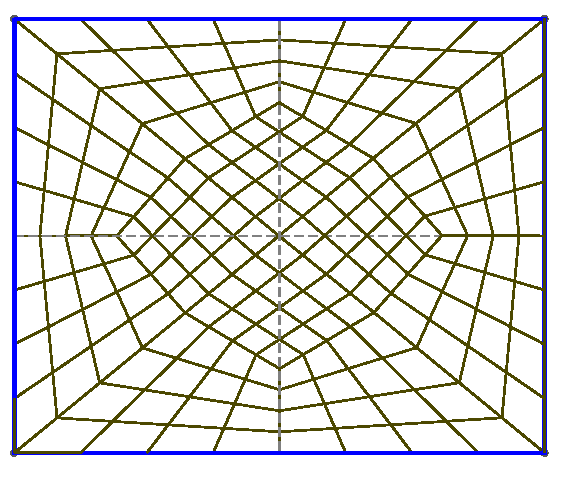
\includegraphics[scale=.6]{images/simple_mesh.pdf}
\caption{GMSH mesh generation example, using Delaunay algorithm.}
\label{fig:simple_mesh}
\end{figure}

\subsubsection{GMSH file format}\label{subsubsection:gmsh_format}
The mesh is stored in a \verb|.msh| file, which is written in \verb|ASCII| format. This type of file is subdivided in sections, which are separated by flags of begin and end.

The first section is mandatory and it starts with the flag \verb|\$MeshFormat|. It contains on the  same row:

\begin{itemize}
\item \textit{version of the format};
\item \textit{type of the file};
\item \textit{data size}.
\end{itemize}

It is ended with the flag \verb|\$EndMeshFormat|.

The second section contains the information on nodes. It begins with the line \verb|\$Nodes|. On the next line there is the total number of nodes,and each of the following lines contains:

\begin{itemize}
\item \textit{global index} of the node;
\item \textit{coordinates} of the node.
\end{itemize}

The section ends with the line \verb|\$EndNodes|.

The next section begins with \verb|\$Elements| and contains the initial points used to build the mesh, the lines connecting these points and the list of elements of the mesh. The first line contains the sum of the total numbers of these three things.  Every element is stored in a line, and for each of them it is possible to find:

\begin{itemize}
\item \textit{global index} of the element;
\item \textit{type of element}: typically this value is 15 for points, 1 for lines, 2 for triangles and 3 for quadrangles;
\item \textit{number of tags}: an integer number which denotes how many of the following numbers are tags which give additional informations;
\item \textit{tags}: by default, the first tag is the number of the physical entity to which the element belongs; the second is the number of the elementary geometrical entity to which the element belongs; for the lines this tag will be used to assign border conditions; the third is the number of mesh partitions to which the element belongs, followed by the partition ids (negative partition ids indicate ghost cells). A zero tag is equivalent to no tag.
\item \textit{global indexes} of the corner nodes of the element.

\end{itemize}

\verb|GMSH| can compute a partition, but we decided to implement our on code to do that, to have more flexibility. Also, the computational cost of the partition is very high, so it is better to perform it on multi processors.

\subsection{METIS}\label{subsection:metis}
\verb|METIS| is a serial software package for partitioning large irregular graphs, partitioning large meshes, and computing fill-reducing orderings of sparse matrices developed at the 	\textit{Department of Computer Science and Engineering} at the \textit{University of Minnesota}.

Since the parallel version, \verb|ParMETIS| is very similar and it is more used in the code, some of the logic behind the algorithms will be explained in the next section. Only the called function will be explained here. For more information cmp. \cite{metis}.

\verb|METIS| is called only to compute neighboring squares for each element using the function \verb|METIS_MeshToDual|. The function contains a quite fast algorithm to compute neighbors, but but we don't know its exact complexity. The function transform a mesh into its dual graph, giving as output the adjacency of the graph. From this it is possible to obtain the neighbors of each element. Inputs of the function are:

\begin{itemize}
\item \verb|ne|, number of elements in the mesh;
\item \verb|nn|, number of nodes in the mesh;
\item \verb|eptr|, \verb|eind|, a pair of arrays storing the mesh. This two arrays are correlated: \verb|eptr| contains indexes of \verb|eind|. \verb|eind| contains global indexes of nodes. The ith element of \verb|eptr| is the index of \verb|eind| from where the nodes of the ith element of the mesh start. So \verb|eind| will contain the node of element $i$ from position \verb|eptr[i]| until position \verb|eptr[i+1]|.
\item \verb|ncommon| specifies the minimum number of nodes that two elements have to be in common to be considered as neighbors. It may be 1 or 2 for quadrangular elements. In this case a value of 1 is used since also the corner neighbors have to be evaluated;
\item \verb|numflag| denotes the style of numbering order. For C-style it has the value of 0, hence here is set to zero.
\end{itemize}

Outputs are:

\begin{itemize}
\item \verb|xadj|,\verb|adjncy|: this two arrays have similar structures of \verb|eptr| and \verb|eind|: the ith value of \verb|xadj| contains the index of \verb|adjncy| where the indexes of the neighboring squares of the ith element start.
\end{itemize}

\subsection{ParMETIS}\label{subsection:parmetis}
The parallel version of \verb|METIS| is \verb|ParMETIS| and it is called to perform the partition optimization. Information about the library are taken from \cite{parmetis}. \verb|ParMETIS| is an \verb|MPI|-based (cmp. Sec.(\ref{subsection:mpi})) parallel library that implements a variety of algorithms for partitioning and repartitioning unstructured graphs and for computing fill-reducing orderings of sparse matrices.

Fig.(\ref{fig:parmetis_diagram}) shows an overview of the functionality provided by \verb|ParMETIS| as well as a guide to its use.

\begin{figure}
\centering
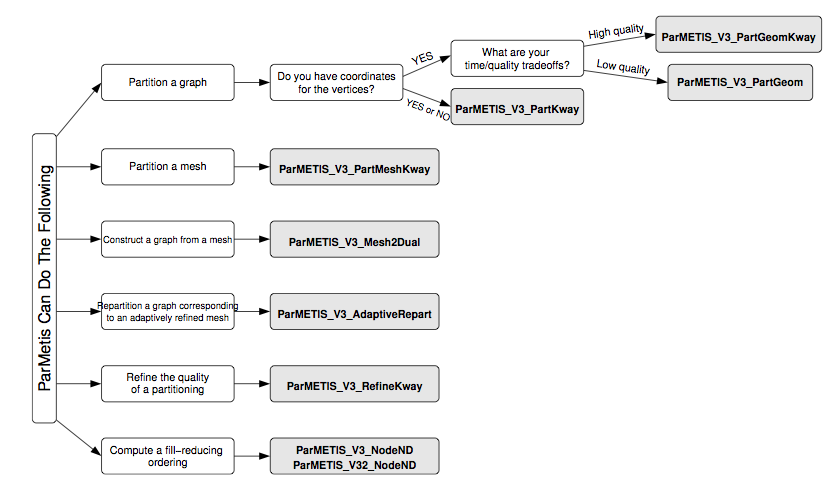
\includegraphics[scale=.45]{images/parmetis.png}
\caption{Functionality of ParMETIS.}
\label{fig:parmetis_diagram}
\end{figure}

The function used to perform the partition optimization is \verb|ParMETIS_V3_PartMeshKway|. Since the algorithm contained in \verb|ParMETIS| can only partition graphs, this function contains a call to \verb|ParMETIS_V3_Mesh2Dual| and then a call to the function \verb|ParMETIS_V3_PartKway|. In this way the dual graph of the mesh is created and then is partitioned using a serial multilevel k-way partitioning algorithm.

This algorithm has been shown to quickly produce partitioning that are of very high quality. It consists of three phases: graph coarsening, initial partitioning, and uncoarsening/refinement. In the graph coarsening phase, a series of graphs is constructed by collapsing together adjacent vertices of the input graph in order to form a related coarser graph. Computation of the initial partitioning is performed on the coarsest (and hence smallest) of these graphs, and so it is very fast. Finally, partition refinement is performed on each level graph, from the coarsest to the finest (i.e., original graph) using a KL/FM-type refinement algorithm.

Fig.(\ref{fig:parmetis_algorithm}) illustrates the multilevel graph partitioning algorithm.

\begin{figure}
\centering
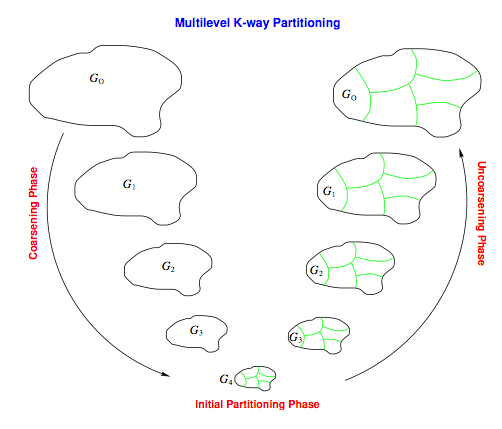
\includegraphics[scale=.45]{images/parmetis_algorithm.png}
\caption{Multilevel K-way partitioning algorithm.}
\label{fig:parmetis_algorithm}
\end{figure}

\verb|ParMETIS_V3_Mesh2Dual| is  used for the refinement. Infact \verb|ParMETIS| can only perform partitioning refinements on graphs, so the sequence \verb|ParMETIS_V3_Mesh2Dual| \verb|ParMETIS_V3_RefineKway| is called for each refinement.

It follows a little explanation of inputs and outputs of the functions used.

\subsubsection{PartMeshKway}\label{subsubsection:partmeshkway}
The function accepts as input a pre-partitioned mesh and returns as output the total number of cut edge in the partition and an array which contains a mapping between elements and processes where they have to be sent.

The pre-partitioned mesh that must be put as input has a different format from the one stored in the code. It is constituted by three arrays:

\begin{itemize}
\item \verb|elmdist| is an array equal in each process and contains the number of elements in each process. The length of \verb|elmdist| is equal to the number of the processes plus one, because each element in \verb|elmdist| denotes the first of the elements on that process, so the last number of \verb|elmdist| is the last element on the last process plus one;
\item \verb|eptr| and \verb|eind| are arrays different in each process. The meaning is exactly the same as described for \verb|METIS| function.
\end{itemize}

The function accepts other inputs:

\begin{itemize}
\item \verb|elmwgt| is a local array of length equal to the length of the local element list and stores the weights for the elements. How this array is obtained will be discussed in detail later.
\item \verb|wgtflag| is a flag which can assume two values: 0 if the partition has to be performed without weights (\verb|elmwgt| is \verb|NULL|), 2 if weights are on vertexes only;
\item \verb|numflag| has the same meaning as in \verb|METIS| function;
\item \verb|ncon| is the number of vertex which every node has (for multiphysics problems);
\item \verb|ncommonnodes| specifies the minimum number of nodes that two elements must have in common to be considered as neighbors. It may be 1 or 2 for quadrangular elements;
\item \verb|nparts| specifies the number of sub-domains desired. In this case it is equal to the number of the processes;
\item \verb|tpwgts| is an array of size \verb|ncon| x \verb|nparts| which specifies the fraction of weights that has to be assigned to each sub-domain. If the distribution has to be uniform each element of this array will have a value of 1/\verb|nparts|;
\item \verb|ubvec| is an array of size \verb|ncon| and specifies the imbalance for each constraint. A value of 1.05 is recommended and used in the code;
\item \verb|options| is an array of integer used to pass some parameters to the routine. Since here this parameters are not used, the first value of options is set to zero and this says to the routine that no options are passed;
\item a pointer to the communicator. Here it is a pointer to \verb|MPI_COMM_WORLD|.
\end{itemize}

The outputs of the function are:

\begin{itemize}
\item \verb|edgecut| contains the number of cut edges;
\item \verb|partition| is an array which contains the ranks of the processes where the elements have to be sent.
\end{itemize}

\subsubsection{Mesh2Dual}\label{subsubsection:mesh2dual}
This function takes in input a mesh with the same format of the previous one, and gives as output the connectivity of the corresponding dual graph. Inputs are:

\begin{itemize}
\item \verb|elmdist|;
\item \verb|eptr|,\verb|eind|;
\item \verb|numflag|;
\item \verb|ncommonnodes|;
\item a pointer to \verb|MPI_COMM_WORLD|.
\end{itemize}

The outputs are the following:

\begin{itemize}
\item \verb|xadj|,\verb|adjncy| with the same meaning as in \verb|METIS| function.
\end{itemize}

\subsubsection{RefineKway}\label{subsubsection:refinekway}
This function take as input a partitioned graph and refines the partition optimizing the number of ghost--cells for each process. As output it gives the rank of the process where each vertex has to be sent. Since the code gives as input the dual graph of a mesh, the output will be the rank of the process where each element (associated to a vertex in the dual graph) has to be sent. As inputs it requires:

\begin{itemize}
\item \verb|vtxdist|: this array has the same function of \verb|elmdist| and specifies how many vertices are stored on each process. The ith element of the array contains the cumulative of the element on the previous processes plus one. The length of the array is equal to the number of the processes plus one;
\item \verb|xadj|,\verb|adjncy|;
\item \verb|vwgt|,\verb|adjwgt| arrays store the weights on vertices and edges;
\item \verb|ncon|;
\item \verb|nparts|;
\item \verb|wgtflag| now can also assume values 1 or 3: 1 if weights are on edges only (\verb|vwgt| is \verb|NULL|), 3 if weights are on both vertices and edges. If it assumes value 2 (weights on vertices only) \verb|adjwgt| is \verb|NULL|;
\item \verb|numflag|;
\item \verb|tpwgts|;
\item \verb|ubvec|;
\item \verb|options|;
\item a pointer to \verb|MPI_COMM_WORLD|.
\end{itemize}

Outputs are:

\begin{itemize}
\item \verb|edgecut|;
\item \verb|partition|;
\end{itemize}

\verb|ParMETIS_V3_RefineKway| can be called repeatedly to further improve the partitioning. However, each successive call will tend to produce smaller improvements in quality.

\subsection{MPI}\label{subsection:mpi}
\verb|MPI| is a \textit{message-passing library interface specification}; for a complete reference to the library cmp. \cite{mpi}. Here we give some information extracted from the manual to explain how the library works. It addresses primarily the message--passing parallel programming model, in which data is moved from the address space of one process to that of another process through cooperative operations on each process. \verb|MPI| is a specification, not an implementation; there are multiple implementations of \verb|MPI|. This specification is for a library interface; \verb|MPI| is not a language, and all \verb|MPI| operations are expressed as functions, subroutines, or methods. It includes point--to--point message--passing, collective communications, group and communicator concepts, process topologies, environmental management, process creation and management, one--sided communications, extended collective operations, external interfaces, I/O, some miscellaneous topics, and a profiling interface.

In the code \verb|MPI| is used to broadcast on each process initial information about the nodes, to send and receive elements information according to different partitioning, and to gather on root process and then send again on each process other information about the partitioning.

All the functions used are blocking. A procedure is blocking if return from the procedure indicates the user is allowed to reuse resources specified in the call. Some functions involve point--to--point communication as  \verb|MPI_Send| and \verb|MPI_Recv|, while the others are collective. The formers may be called only on particular processes, while the latter have to be called at the same moment on each process of the same communicator. Collective calls over the same communicator must be executed in the same order by all members of the process group.

It follows a short explanation of all the functions used.

\subsubsection{MPI\_Send}\label{subsubsection:send}
\verb|MPI_Send| is a point--to--point blocking function. It is used to send data from a particular process to another particular one. It accepts the following inputs:

\begin{itemize}
\item \verb|buf|, the initial address of send buffer;
\item \verb|count|, number of elements in send buffer;
\item \verb|datatype|, type of each send buffer elements (\verb|MPI_DATATYPE|);
\item \verb|dest|, rank of destination;
\item \verb|tag|, message tag (integer);
\item \verb|comm|, \verb|MPI| communicator.
\end{itemize}

\subsubsection{MPI\_Recv}\label{subsubsection:recv}
Each time data are sent to a specific process this process must call this function to receive the buffer of data. The function accepts the followings:

\begin{itemize}
\item \verb|buf|, the initial address of send buffer;
\item \verb|count|, number of elements in send buffer;
\item \verb|datatype|, type of each send buffer elements (\verb|MPI_DATATYPE|);
\item \verb|source|, rank of source or \verb|MPI_ANY_SOURCE|;
\item \verb|tag|, message tag or \verb|MPI_ANY_TAG| (integer);
\item \verb|comm|, \verb|MPI| communicator;
\end{itemize}

Outputs are:

\begin{itemize}
\item \verb|buf|, the initial address of send buffer;
\item \verb|status|, status object.
\end{itemize}

\subsubsection{MPI\_Bcast}\label{subsubsection:bcast}
\verb|MPI_Bcast| is a collective blocking function. It's goal is to send the same data from a single process to each process of the communicator. The logic is outlined in Fig.(\ref{fig:bcast}).

\begin{figure}
\centering
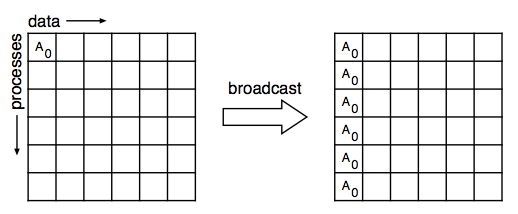
\includegraphics[scale=.45]{images/broadcast.png}
\caption{MPI\_Bcast logic.}
\label{fig:bcast}
\end{figure}

The function accepts the followings:

\begin{itemize}
\item \verb|buf|, starting address of the buffer; it is an input on root processor and an output on the other ones.
\item \verb|count|, number of elements in buffer;
\item \verb|datatype|, type of each send buffer elements (\verb|MPI_DATATYPE|);
\item \verb|root|, rank of broadcast root;
\item \verb|comm|, \verb|MPI| communicator.
\end{itemize}

\subsubsection{MPI\_Scatter}\label{subsubsection:scatter}
\verb|MPI_Scatter| is a collective blocking function. It is used to send from root process to each other process a different part of a buffer. All the parts have the same size. The logic and the one of gather function are specified in Fig.(\ref{fig:scatter_gather}).
\begin{figure}
\centering
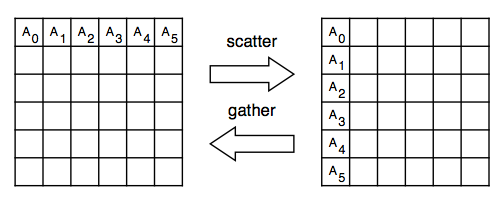
\includegraphics[scale=.45]{images/scatter_gather.png}
\caption{MPI\_Bcast logic.}
\label{fig:scatter_gather}
\end{figure}

The function requires the followings:

\begin{itemize}
\item \verb|sendbuf|, address of send buffer;
\item \verb|sendcount|, number of elements send to each process;
\item \verb|sendtype|, type of each sent buffer elements (\verb|MPI_DATATYPE|);
\item \verb|recvbuf|, address of receive buffer;
\item \verb|recvcount|, number of elements in receive buffer;
\item \verb|recvtype|, data type of receive buffer elements (\verb|MPI_DATATYPE|);
\item \verb|root|, rank of broadcast root;
\item \verb|comm|, \verb|MPI| communicator.
\end{itemize}

The output is:

\begin{itemize}
\item \verb|recvbuf|, address of receive buffer;
\end{itemize}

\subsubsection{MPI\_Scatterv}\label{subsubsection:scatterv}
It has the same logic of \verb|MPI_Scatter|, but it is possible to specify how many elements send to each process. Only two parameters change from the previous function:

\begin{itemize}
\item \verb|sendcounts|, non-negative integer array (of length group size) specifying the number of elements to send to each rank;
\item \verb|displs|, integer array(of length group size). Entry i specifies the displacement (relative to \verb|sendbuf|) from which to take the outgoing data to process $i$.
\end{itemize}

\subsubsection{MPI\_Gather}\label{subsubsection:gather}
This function has the goal to gather data coming from different processes on a single process. The logic is shown in Sec.(\ref{subsubsection:scatter}) paragraph. It accepts the same parameters as \verb|MPI_Scatter|.

A further explanation is given in Fig.(\ref{fig:gather})

\begin{figure}
\centering
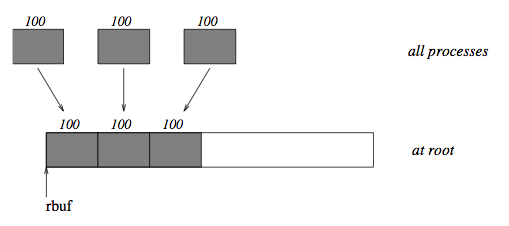
\includegraphics[scale=.45]{images/gather.png}
\caption{MPI\_Gather logic.}
\label{fig:gather}
\end{figure}

\subsection{PETSc}\label{subsection:PETSc}
\verb|PETSc|, \textit{Portable, Extensible Toolkit for Scientific Computation} is a suite of data structures and routines that provide the building blocks for the implementation of large scale application codes on parallel (and serial) computers. The information reported here are taken from \cite{petsc}. Compare it for additional guidelines.

It is a hierarchically organized library, which, by using an object-oriented programming, enables users  to employ the level of abstraction that is most appropriate for a particular problem, providing enormous flexibility. \verb|PETSc| uses \verb|MPI| standard for all message-passing communication.

The library contains modules to deal with:

\begin{itemize}
\item index sets (\verb|IS|), including permutations, for indexing into vectors, renumbering, etc;
\item vectors (\verb|Vec|);
\item matrices (\verb|Mat|) (generally sparse);
\item managing interactions between mesh data structures and vectors and matrices (\verb|DM|);
\item over fifteen Krylov subspace methods (\verb|KSP|);
\item dozens of preconditioners, including multi-grid, block solvers, and sparse direct solvers (\verb|PC|);
\item nonlinear solvers (\verb|SNES|);
\item time steppers for solving time-dependent (nonlinear) PDEs, including support for differential algebraic equations (\verb|TS|).
\end{itemize}

In this section we explain the functions used in the class \verb|ghost_communication|.

\subsubsection{VecCreate}\label{subsubsection:VecCreate}
This is the general function to create an empty vector without any type. Input parameters:

\begin{itemize}
\item \verb|comm| - the communicator for the vector object.
\end{itemize}
Output parameters:
\begin{itemize}
\item \verb|vec| - a pointer to the vector object.
\end{itemize}

\subsubsection{VecCreateGhost}\label{subsubsection:VecCreateGhost}
Creates a parallel vector with ghost padding on each processor. Input parameters:

\begin{itemize}
\item \verb|comm| - the communicator to use;
\item \verb|n| - local vector length;
\item \verb|N| - global vector length (or \verb|PETSC_DECIDE| if \verb|n| is given);
\item \verb|nghost| - number of local ghost points;
\item \verb|ghosts| - array of global indices of ghost points.
\end{itemize}

Output parameters:

\begin{itemize}
\item \verb|vv| - a pointer to the global vector representation (without ghost points as part of vector).
\end{itemize}

\subsubsection{VecSetValues}\label{subsubsection:VecSetValues}
Inserts or adds values into certain locations of a vector. Input parameters:

\begin{itemize}
\item \verb|x| - vector to insert in;
\item \verb|ni| - number of elements to add;
\item \verb|ix| - array of indexes where to add;
\item \verb|y| - array of values;
\item \verb|iora| - insert mode (\verb|INSERT_VALUES| or \verb|ADD_VALUES|).
\end{itemize}

\subsubsection{VecAssemblyBegin and VecAssemblyEnd}\label{subsubsection:VecAssembly}
The former begins and the latter ends to assembly a vector. This routines should be called in sequence after completing a call to \verb|VecSetValues|. Input parameters:

\begin{itemize}
\item \verb|vec| - the vector.
\end{itemize}

\subsubsection{VecGhostUpdateBegin and VecGhostUpdateEnd}\label{subsubsection:VecGhostUpdate}
The former begins and the latter ends the vector scatter to update the vector from local representation to global or global representation to local. They should be called in sequence after having updated the local or global vector. Input parameters:

\begin{itemize}
\item \verb|g| - the vector;
\item \verb|insertmode| - \verb|ADD_VALUES| or \verb|INSERT_VALUES|;
\item \verb|scattermode| - \verb|SCATTER_FORWARD| or \verb|SCATTER_REVERSE|.
\end{itemize}

\subsubsection{VecGhostGetLocalForm and VecGhostRestoreLocalForm}\label{subsubsection:VecGhostGetLocalForm}
Obtains the local ghosted representation of a parallel vector. Input parameters:

\begin{itemize}
\item \verb|g| - the global vector.
\end{itemize}
\begin{itemize}
\item \verb|l| -a pointer to the local ghosted representation.
\end{itemize}

\subsubsection{VecGhostRestoreLocalForm}\label{subsubsection:VecGhostRestoreLocalForm}
Restores the local ghosted representation of a parallel vector after being used. Input parameters:

\begin{itemize}
\item \verb|g| - the global vector;
\item \verb|l| - a pointer to the local ghosted representation.
\end{itemize}

\subsubsection{VecGetValues}\label{subsubsection:VecGetValues}
Gets values from certain locations of a vector. Can only get values on the same processor. Input parameters:

\begin{itemize}
\item \verb|x| - vector to get the values from;
\item \verb|ni| - number of elements to get;
\item \verb|ix| - array of indices where to get them from (in global 1d numbering).
\end{itemize}

Output parameters:

\begin{itemize}
\item \verb|y| - array of values.
\end{itemize}

\subsubsection{PetscFree}\label{subsubsection:PetscFree}
Frees memory. Input parameters:

\begin{itemize}
\item \verb|memory| - memory to free.
\end{itemize}

\subsubsection{VecDestroy}\label{subsubsection:VecDestroy}
Destroys a vector. Input parameters:

\begin{itemize}
\item \verb|v| - a pointer to the vector.
\end{itemize}

\section{Examples}\label{section:mesh_ex}
Now we report two examples in which we test the performance of this part of the code. In the first example, Sec.(\ref{subsection:Tokamak_section}) we mesh the Scrape of Layer (SOL) and the internal part of the toroidal section of a Tokamak.In the second one, Sec.(\ref{subsection:mirror_machine}) we mesh the interior part of the mirror machine following the magnetic field lines.

\subsection{Tokamak section}\label{subsection:Tokamak_section}
As explained previously (cmp. Sec(\ref{subsection:gmsh})) \verb|GMSH| allows the user to build the mesh on the domain using different algorithms; in particular it's possible to choose as option an algorithm based on a \textit{frontal} approach, or a \textit{Delaunay} or a \textit{mesh adaptation} one. As it is possible to see in Fig.(\ref{fig:mesh}) the density of elements is higher in the upper  and the lower part of the domain: this is due to the fact \verb|GMSH| builds an higher number the elements where the density of points on the border of the domain is higher. In this particular example the \textit{frontal} and the \textit{mesh adaptation} algorithms seem to build a mesh in which the distribution of elements is more uniform.
\medskip

In the following figures the part of the code regarding the management of the grid as been run on four process using a finer grid (11746 elements) built using a mesh adaptation algorithm. The Fig.(\ref{fig:prepartitioning}) shows the results obtained at the first step of the distribution of the elements on the processes pre-partitioning as been implemented simply dividing the list of elements in almost equal part on each process. GMSH creates a pseudo-random numbering of the elements: so, on each process, a disjointed domain is created (cmp Fig.(\ref{fig:prepartitioning})). In Fig.(\ref{fig:partitioning}) the new redistribution of elements among processes is reported: on each process part the domain is reconstructed using \verb|ParMetis|, creating a non-disjointed domain. The four domain seem to be different: the partitioning has been constructed using a uniform distribution of the \verb|weights|, so almost the same number of elements has been associated to each processor. In the last Fig.(\ref{fig:refinement}) we performed 5 refinements of the mesh partitioning.

\begin{figure}
\centering
\subfigure[{Frontal: 4197 elements}\label{fig:tokamak_layer_frontal}]
{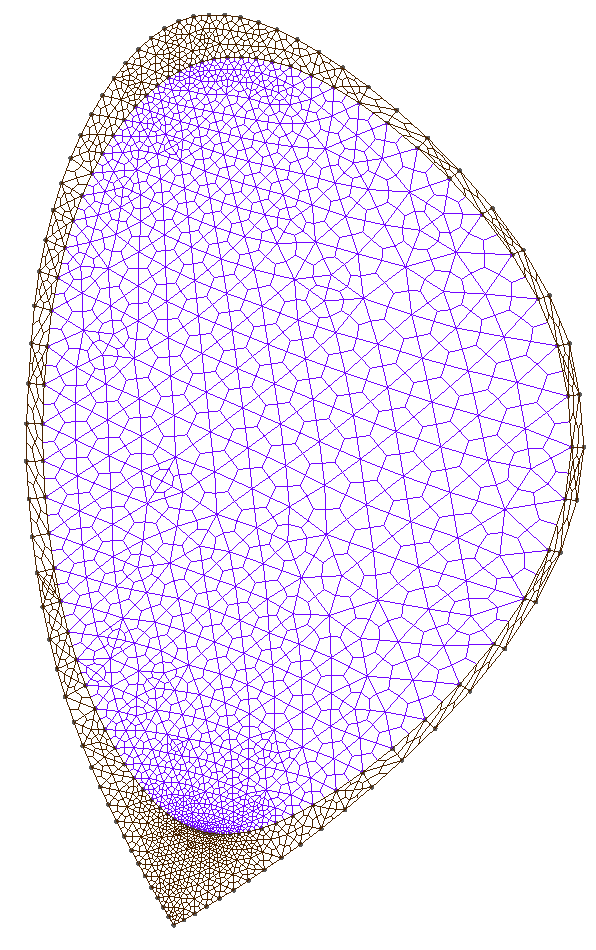
\includegraphics[scale=.55]{images/tokamak_layer_frontal.pdf}}\quad\quad
\subfigure[{Delaunay: 4803 elements.}\label{fig:tokamak_layer_delaunay}]
{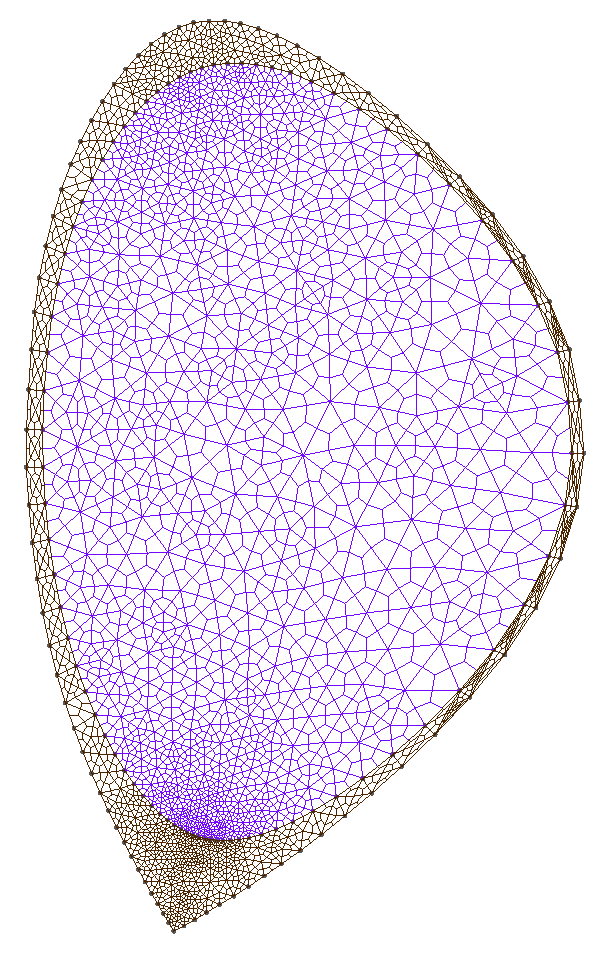
\includegraphics[scale=.55]{images/tokamak_layer_delaunay.pdf}}\quad\quad
\subfigure[{Mesh adaptation: 3213 elements}\label{fig:tokamak_layer_mesh_adapt}]
{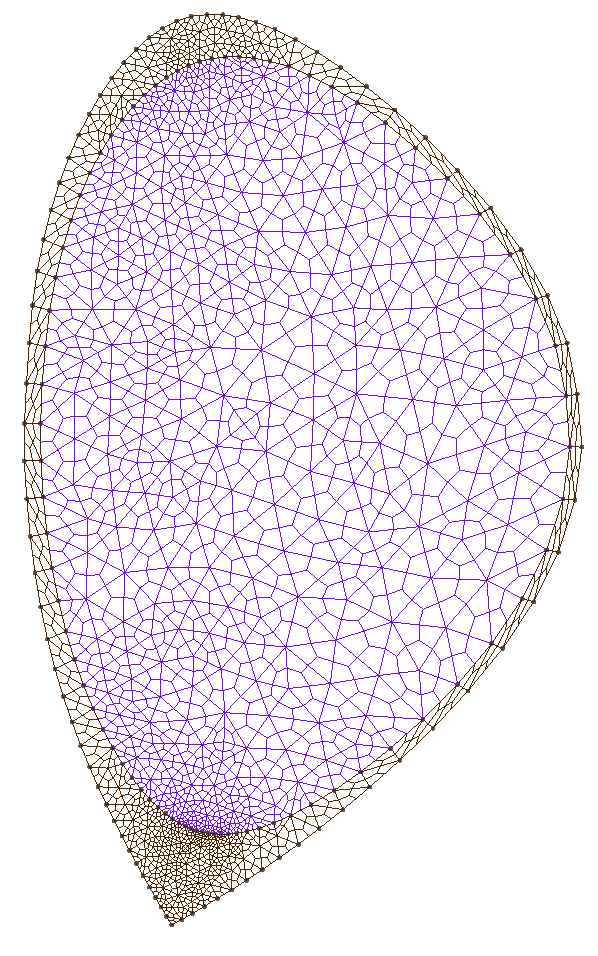
\includegraphics[scale=.55]{images/tokamak_layer_mesh_adapt.pdf}}
\caption{Mesh creation options of a Tokamak section.}\label{fig:mesh}
\end{figure}

\begin{figure}
\centering
\subfigure[{rank = 0}\label{fig:tokamak_layer_mesh_adapt_fine_0_pre}]
{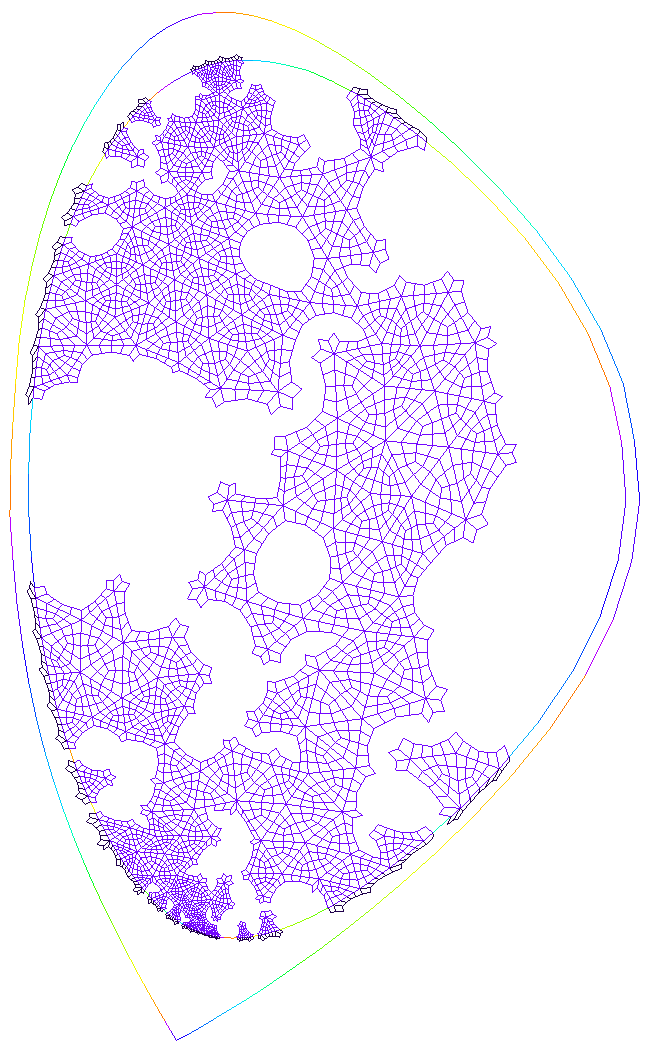
\includegraphics[scale=.5]{images/tokamak_layer_mesh_adapt_fine_0_pre.pdf}}\quad
\subfigure[{rank = 1}\label{fig:tokamak_layer_mesh_adapt_fine_1_pre}]
{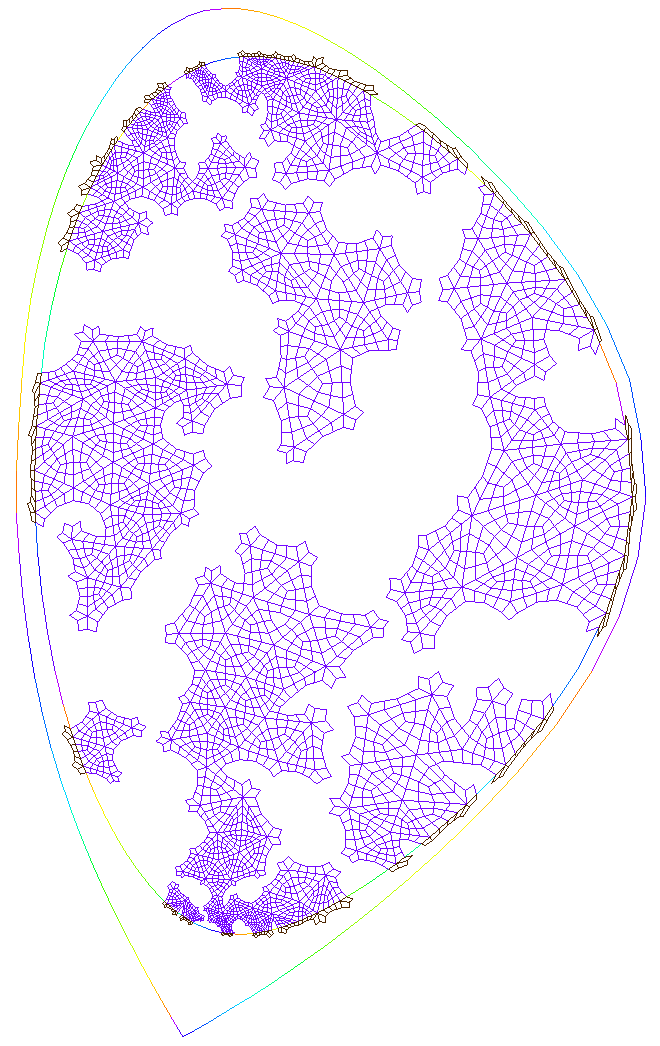
\includegraphics[scale=.5]{images/tokamak_layer_mesh_adapt_fine_1_pre.pdf}}\quad
\subfigure[{rank = 2}\label{fig:tokamak_layer_mesh_adapt_fine_2_pre}]
{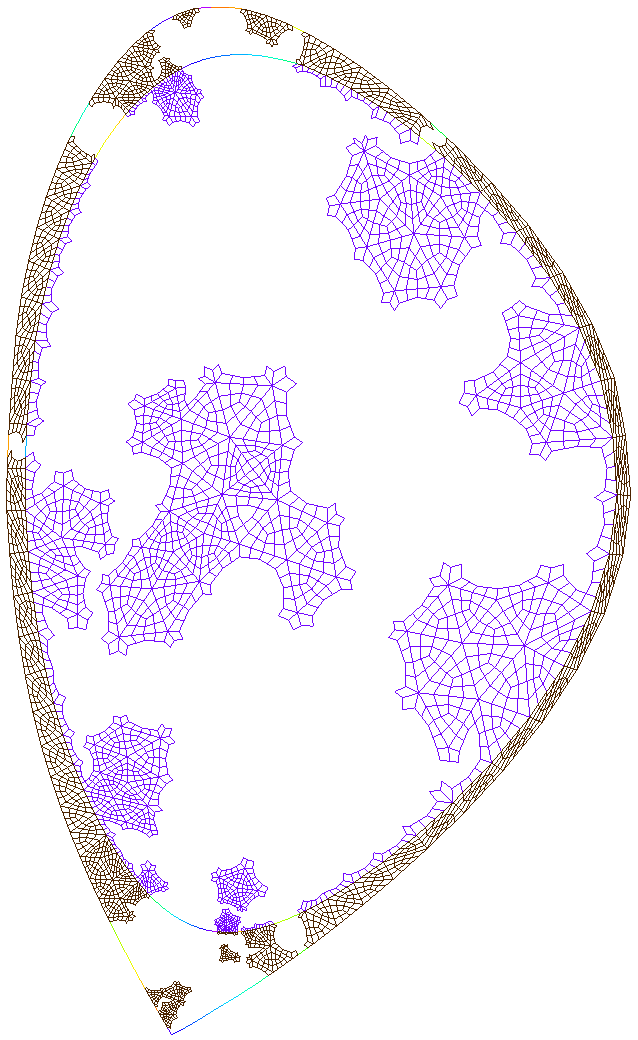
\includegraphics[scale=.5]{images/tokamak_layer_mesh_adapt_fine_2_pre.pdf}}\quad
\subfigure[{rank = 3}\label{fig:tokamak_layer_mesh_adapt_fine_3_pre}]
{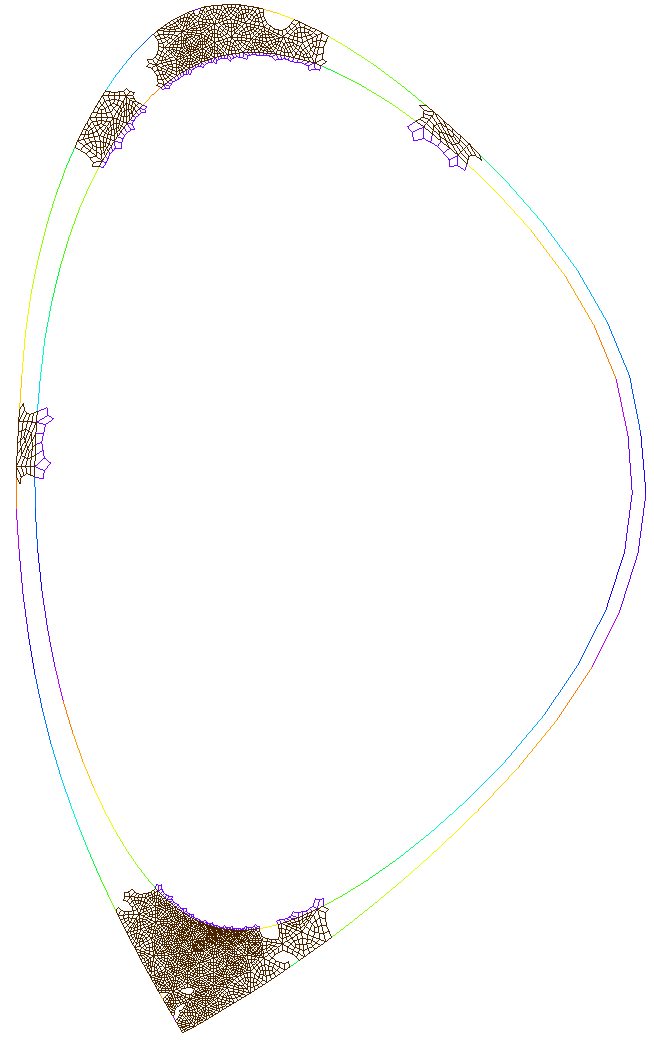
\includegraphics[scale=.5]{images/tokamak_layer_mesh_adapt_fine_3_pre.pdf}}\quad
\caption{Prepartitioning of a Tokamak section.}\label{fig:prepartitioning}
\end{figure}

\begin{figure}
\centering
\subfigure[{rank = 0}\label{fig:tokamak_layer_mesh_adapt_fine_0_par}]
{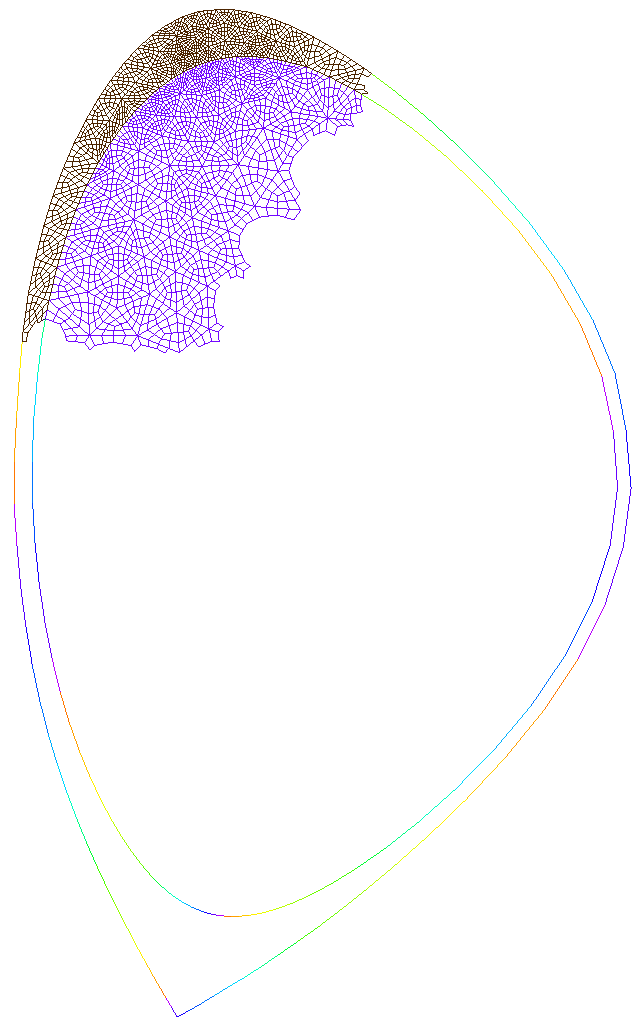
\includegraphics[scale=.5]{images/tokamak_layer_mesh_adapt_fine_0_par.pdf}}\quad
\subfigure[{rank = 1}\label{fig:tokamak_layer_mesh_adapt_fine_1_par}]
{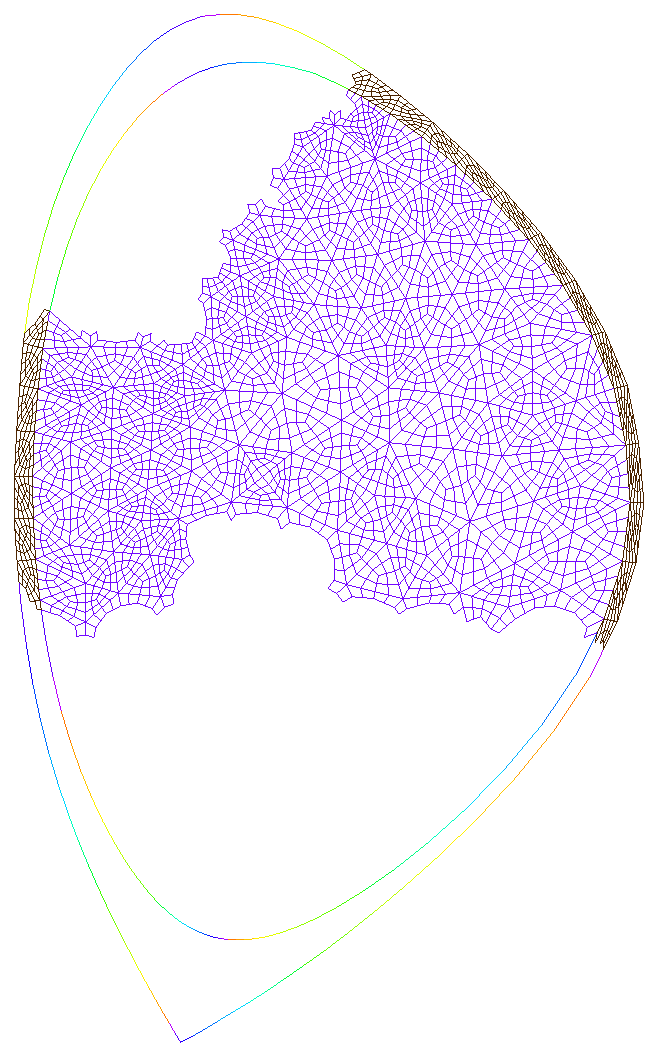
\includegraphics[scale=.5]{images/tokamak_layer_mesh_adapt_fine_1_par.pdf}}\quad
\subfigure[{rank = 2}\label{fig:tokamak_layer_mesh_adapt_fine_2_par}]
{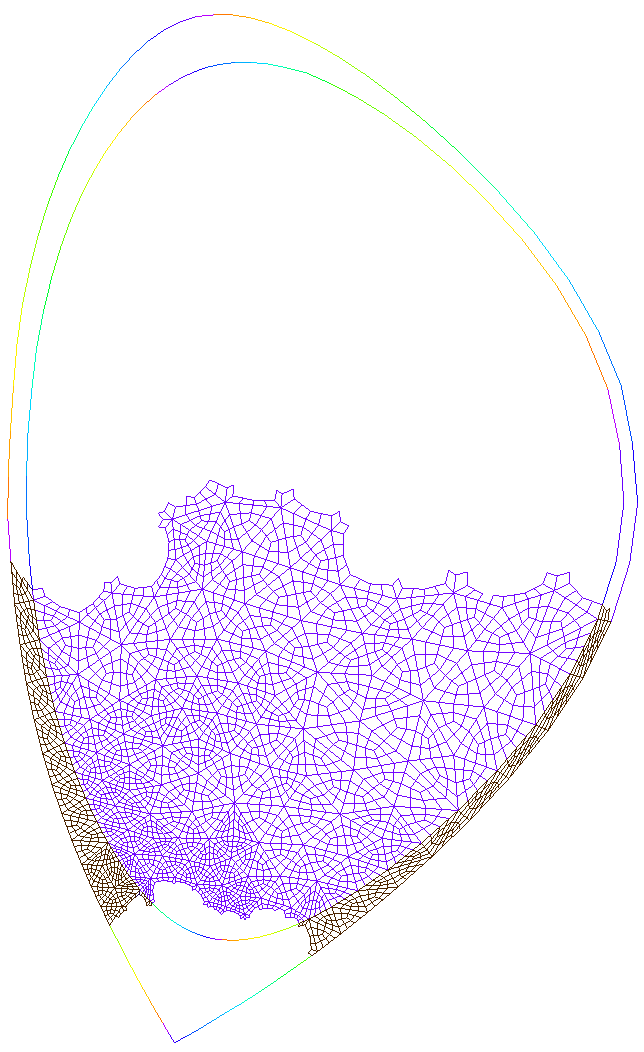
\includegraphics[scale=.5]{images/tokamak_layer_mesh_adapt_fine_2_par.pdf}}\quad
\subfigure[{rank = 3}\label{fig:tokamak_layer_mesh_adapt_fine_3_par}]
{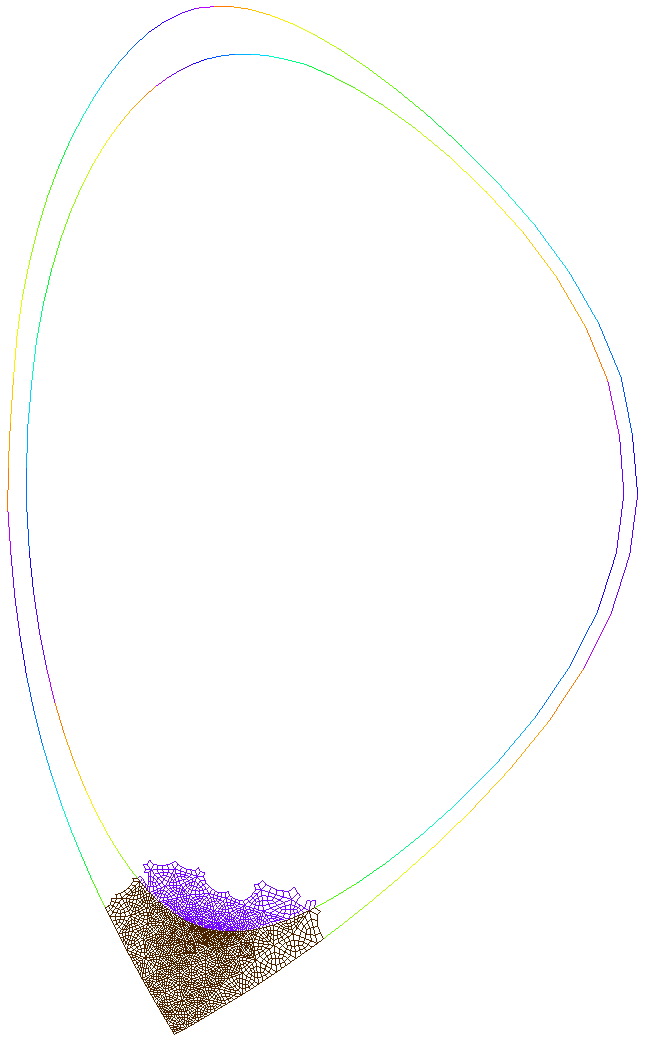
\includegraphics[scale=.5]{images/tokamak_layer_mesh_adapt_fine_3_par.pdf}}\quad
\caption{Partitioning of a Tokamak section.}\label{fig:partitioning}
\end{figure}

\begin{figure}
\centering
\subfigure[{rank = 0}\label{fig:tokamak_layer_mesh_adapt_fine_0_ref}]
{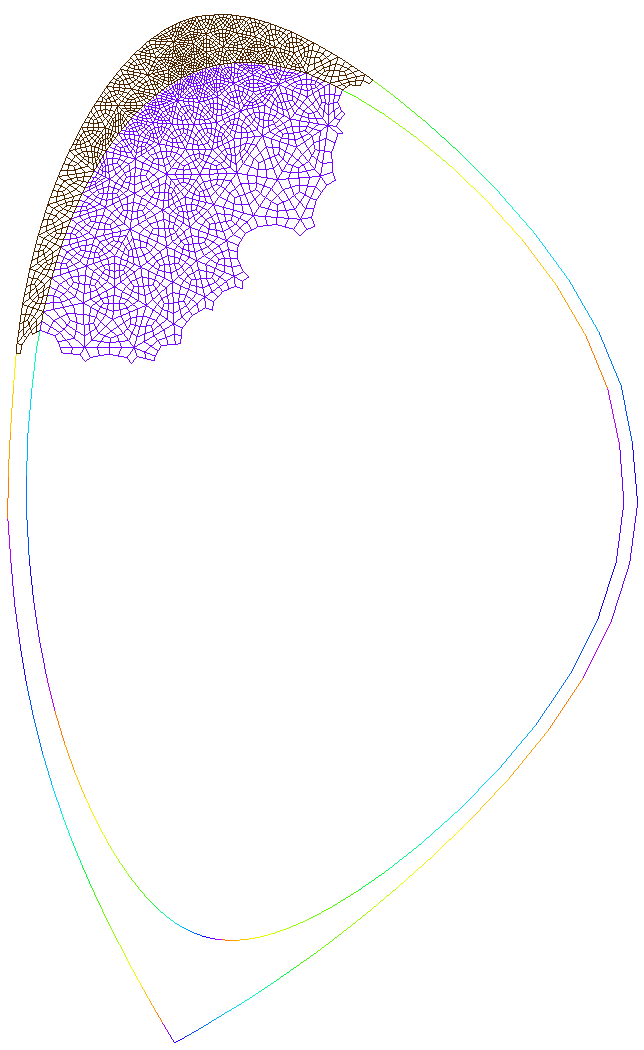
\includegraphics[scale=.5]{images/tokamak_layer_mesh_adapt_fine_0_ref.pdf}}\quad
\subfigure[{rank = 1}\label{fig:tokamak_layer_mesh_adapt_fine_1_ref}]
{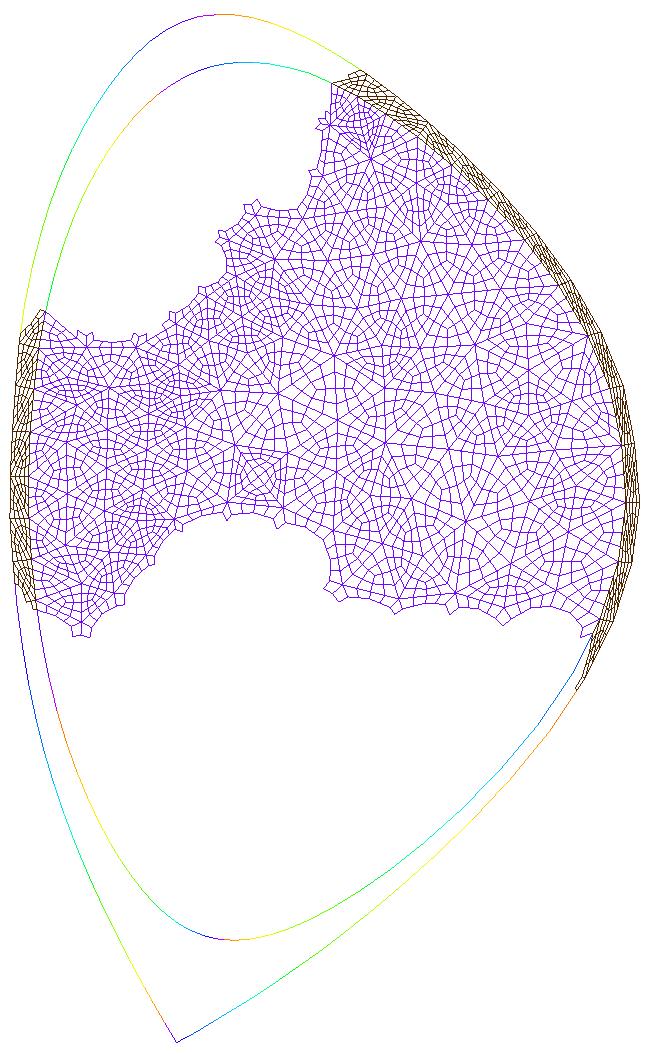
\includegraphics[scale=.5]{images/tokamak_layer_mesh_adapt_fine_1_ref.pdf}}\quad
\subfigure[{rank = 2}\label{fig:tokamak_layer_mesh_adapt_fine_2_ref}]
{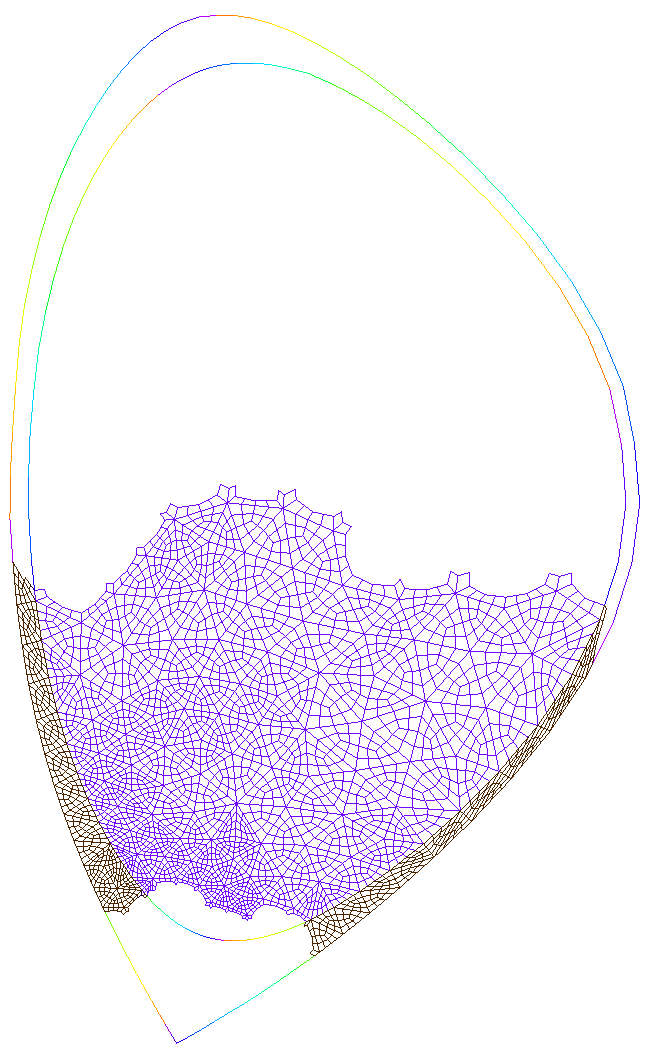
\includegraphics[scale=.5]{images/tokamak_layer_mesh_adapt_fine_2_ref.pdf}}\quad
\subfigure[{rank = 3}\label{fig:tokamak_layer_mesh_adapt_fine_3_ref}]
{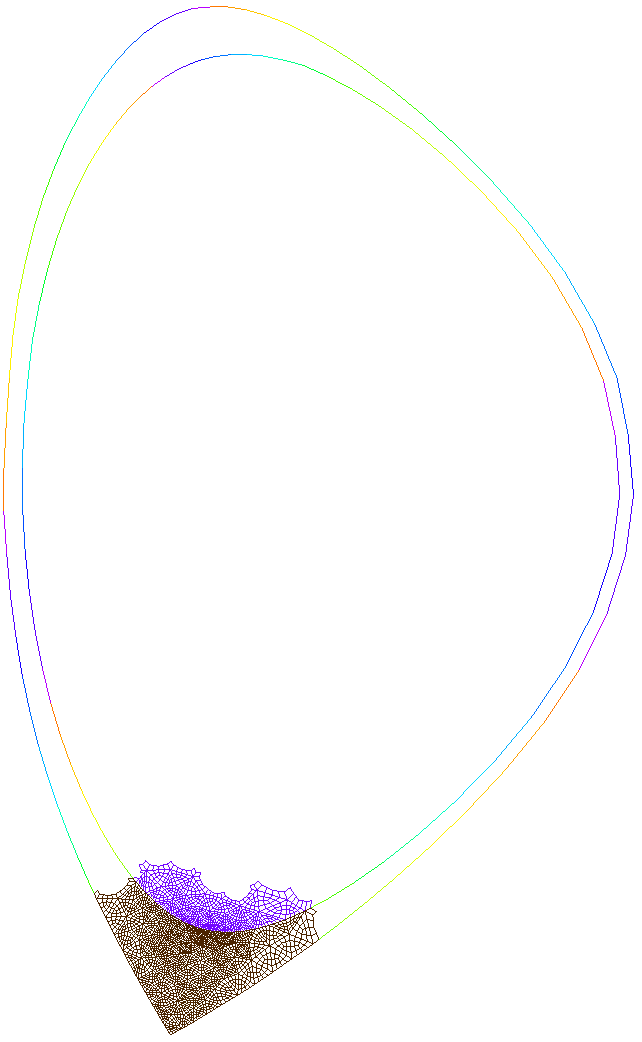
\includegraphics[scale=.5]{images/tokamak_layer_mesh_adapt_fine_3_ref.pdf}}\quad
\caption{5 refinements of a Tokamak section.}\label{fig:refinement}
\end{figure}
\newpage

\subsection{Mirror machine section}\label{subsection:mirror_machine}
In Fig.(\ref{fig:mirror}) we report the meshed section of the magnetic fields lines inside a mirror machine; this mesh is partitioned over 8 processes, indicated by different colors.

\begin{table}
\centering
\begin{tabular}{|c|c|c|}
\hline
 N. Refinements & Time (s) & N. Ghosts\\
\hline
 0 & 0.23 & 163\\
\hline
 1 &  0.28 & 155\\
\hline
 2 & 0.35 & 153\\
\hline
 3 & 0.42 & 153\\
\hline
 4 & 0.49 & 153\\
\hline
 5 & 0.55 & 153\\
\hline
\end{tabular}
\caption{Mirror machine ($3.6\cdot 10^{4}$ elements).}
\label{tab:mirror_36k}
\end{table}

We compare the performances, in terms of execution time and reduction of number of ghosts, of \verb|ParMETIS| refine algorithm. In Tab.(\ref{tab:mirror_36k}) we use a mesh of $3.6\cdot 10^{4}$ elements starting from 0 refinements until 5 refinements. We can notice that the average number of ghosts slightly reduces with the first two refinements and after it remains constant: the improvement is about 6\%, so the parallel communication is reduced of the same amount. It is worth to compare the time of execution with a larger grid. In fact, while in the small grid case the time of execution is influenced mainly by the reading and partitioning, then each refinement contributes by a fraction of the total time, in the second case (cmp. Tab.(\ref{tab:mirror_26M})) every refinement takes almost three times the time spent in the first part. This means that the complexity of the refinement algorithm is not linear. The final improvement after 5 refinements is 6.5\%.

\begin{table}
\centering
\begin{tabular}{|c|c|c|}
\hline
 N. Refinements & Time (s) & N. Ghosts\\
\hline
 0 & 63.43 & 1369\\
\hline
 1 &  242.23 & 1319\\
\hline
 2 & 418.63 & 1300\\
\hline
 3 & 604.96 & 1292\\
\hline
 4 & 778.94 & 1285\\
\hline
 5 & 956.44 & 1280\\
\hline
\end{tabular}
\caption{Mirror machine ($2.6\cdot 10^{6}$ elements).}
\label{tab:mirror_26M}
\end{table}

\begin{figure}
\centering
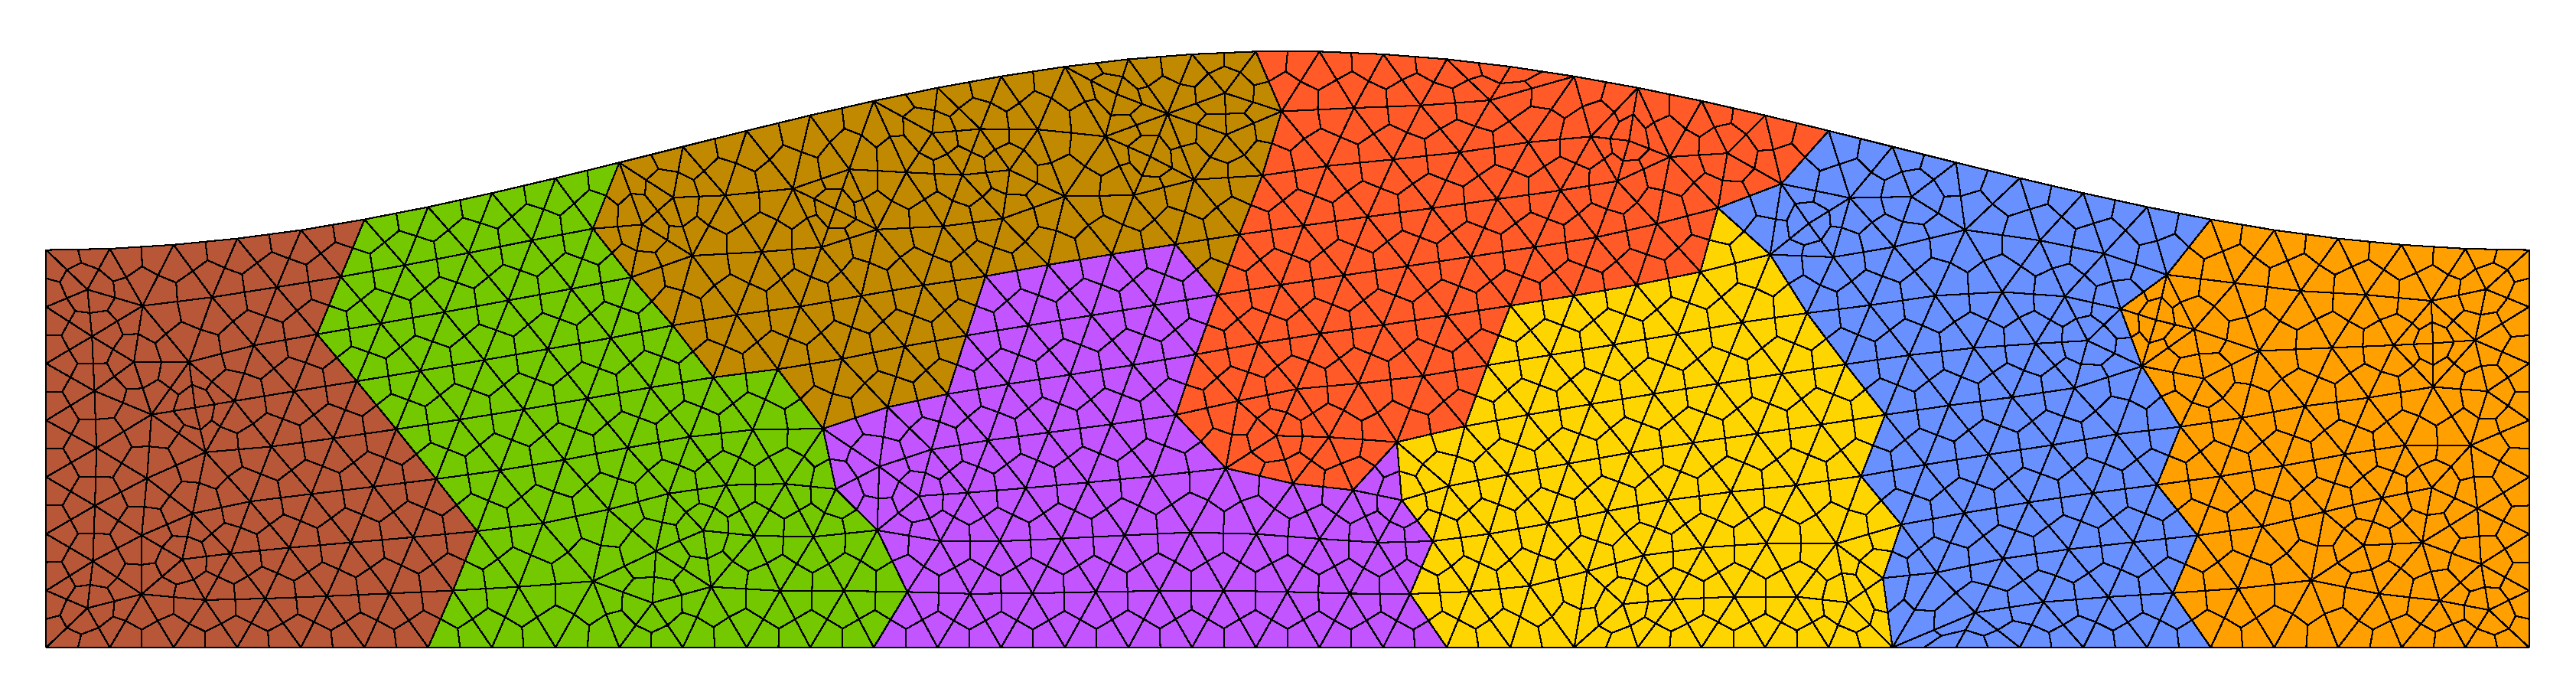
\includegraphics[scale=.27]{images/mirror_partitioned.eps}
\caption{Partitioning of a mirror machine section (2350 elements).}
\label{fig:mirror}
\end{figure}
